\appendix
\chapter{Security Implementation}
\definecolor{codegreen}{rgb}{0,0.6,0}
\definecolor{codegray}{rgb}{0.5,0.5,0.5}
\definecolor{codepurple}{rgb}{0.58,0,0.82}
\colorlet{backcolour}{gray!10}
\definecolor{constcolor}{RGB}{59,130,246} % Blue for 'const'
\definecolor{exportcolor}{RGB}{168,85,247} % Purple for 'export'

\lstset{
    emph={const}, emphstyle={\color{constcolor}}, % Blue for const
    emph={[2]export}, emphstyle={[2]\color{exportcolor}}, % Purple for export
}

\lstdefinestyle{typescript}{
    backgroundcolor=\color{backcolour},   
    commentstyle=\color{codegreen},
    keywordstyle=\color{magenta},
    numberstyle=\tiny\color{codegray},
    stringstyle=\color{codepurple},
    basicstyle=\ttfamily\footnotesize,
    breakatwhitespace=false,
    breaklines=true,
    captionpos=b,
    keepspaces=true,
    numbers=left,
    numbersep=5pt,
    showspaces=false,
    showstringspaces=false,
    showtabs=false,
    tabsize=2,
    morekeywords={export,const}, % Add export and const as keywords
    language=JavaScript % TypeScript is not directly supported, but JavaScript is close enough
}



\begin{lstlisting}[style=typescript,caption=Input Validation,label=apendix:input_val]
import {z} from "zod";

export const authorizationSchema = z.object({
    response_type: z.literal('code').optional() ,
    username: z.string(),
    password: z.string(),
    client_id: z.string(),
    redirect_uri: z.string().url().optional() ,
    scope: z.string().optional() ,
    state: z.string().optional() ,
    codeChallenge: z.string(),
    code_challenge_method: z.literal('S256').optional() ,
});

export const tokenRequestSchema = z.object({
    grant_type: z.literal('authorization_code'),
    authorizationCode: z.string(),
    redirect_uri: z.string().url().optional(),
    client_id: z.string(),
    codeVerifier: z.string()
});

\end{lstlisting}

\newpage
\begin{lstlisting}[style=typescript,caption=Code Challenge Validation,label=apendix:code_chal_val]
export const isCodeChallengeValid = (data: string): boolean => {
    const validLength = data.length >= 43 && data.length <= 128;
    // This code challenge is base64url encoded
    const validCharset = /^[A-Za-z0-9-._~]+$/.test(data);
    return validLength && validCharset;
}
\end{lstlisting}

\begin{lstlisting}[style=typescript,caption=Code Challenge Timing safe comparisons,label=apendix:timing_safe_comparions]
import crypto from 'crypto';

export const verifySHA = async (toVerify: string, expectedHash: string): Promise<boolean> => {
    const hash = await sha256(toVerify);
    // convert the hash to base64 url safe encoding without padding
    const base64Hash = Buffer.from(hash, 'hex').toString('base64').replace(/=+$/, '').replace(/\+/g, '-').replace(/\//g, '_');
    // prevent timing attacks by using crypto.timingSafeEqual
    return crypto.timingSafeEqual(Buffer.from(base64Hash), Buffer.from(expectedHash));
};
\end{lstlisting}

\newpage

\begin{lstlisting}[style=typescript,caption=Token Signature using Assymetric key with RS256 stored in Secrets Manager,label=apendix:token_signing]
import { SecretsManagerClient, GetSecretValueCommand } from '@aws-sdk/client-secrets-manager';
const client = new SecretsManagerClient({ region: 'us-east-1' });
export const getSecret = async (secretName: string): Promise<string> => {
    try {
        const command = new GetSecretValueCommand({ SecretId: secretName });
        const data = await client.send(command);
        if (data && data.SecretString) {
            return data.SecretString;
        } else {
            throw new Error('Secret binary data is not supported');
        }
    } catch (error) {
        console.error(`Error retrieving secret ${secretName}:`, error);
        throw error;
    }
};

// Load the private key from Secrets Manager
const privateKey = await getSecret('private_key');
// Generate JWT token
const token = jwt.sign(
    {
        userId: data.Items[0].id.S
    },
    privateKey, // Replace with your secret key
    {
        expiresIn: '1h',
        algorithm: 'RS256',
    }
);

\end{lstlisting}

\begin{figure}[h!]
\label{fig:argon2id_hash}
\centering
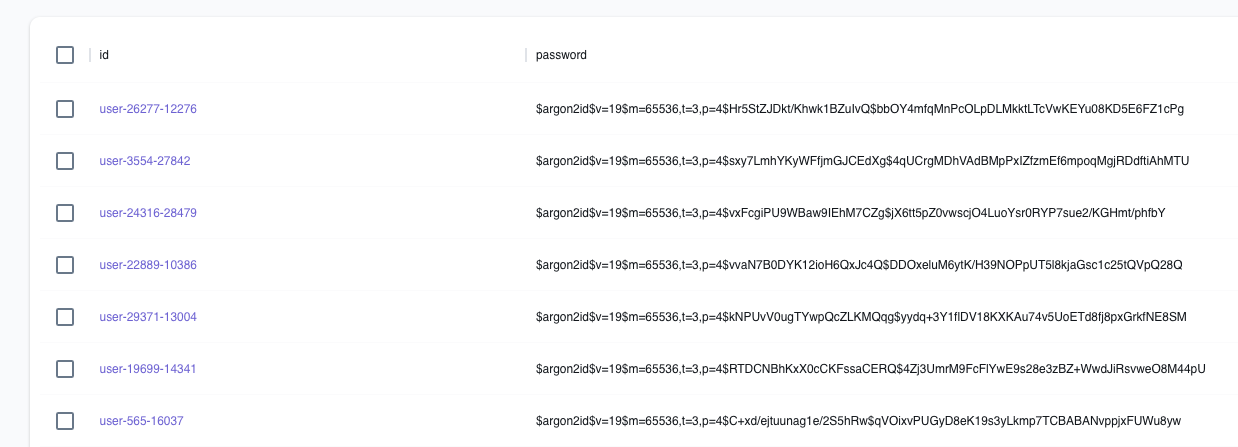
\includegraphics[width=\textwidth, height=200px]{pics/argon2id.png}
\caption{User Passwords hashed with Argon2id}
\end{figure}

\begin{figure}[!htbp]
    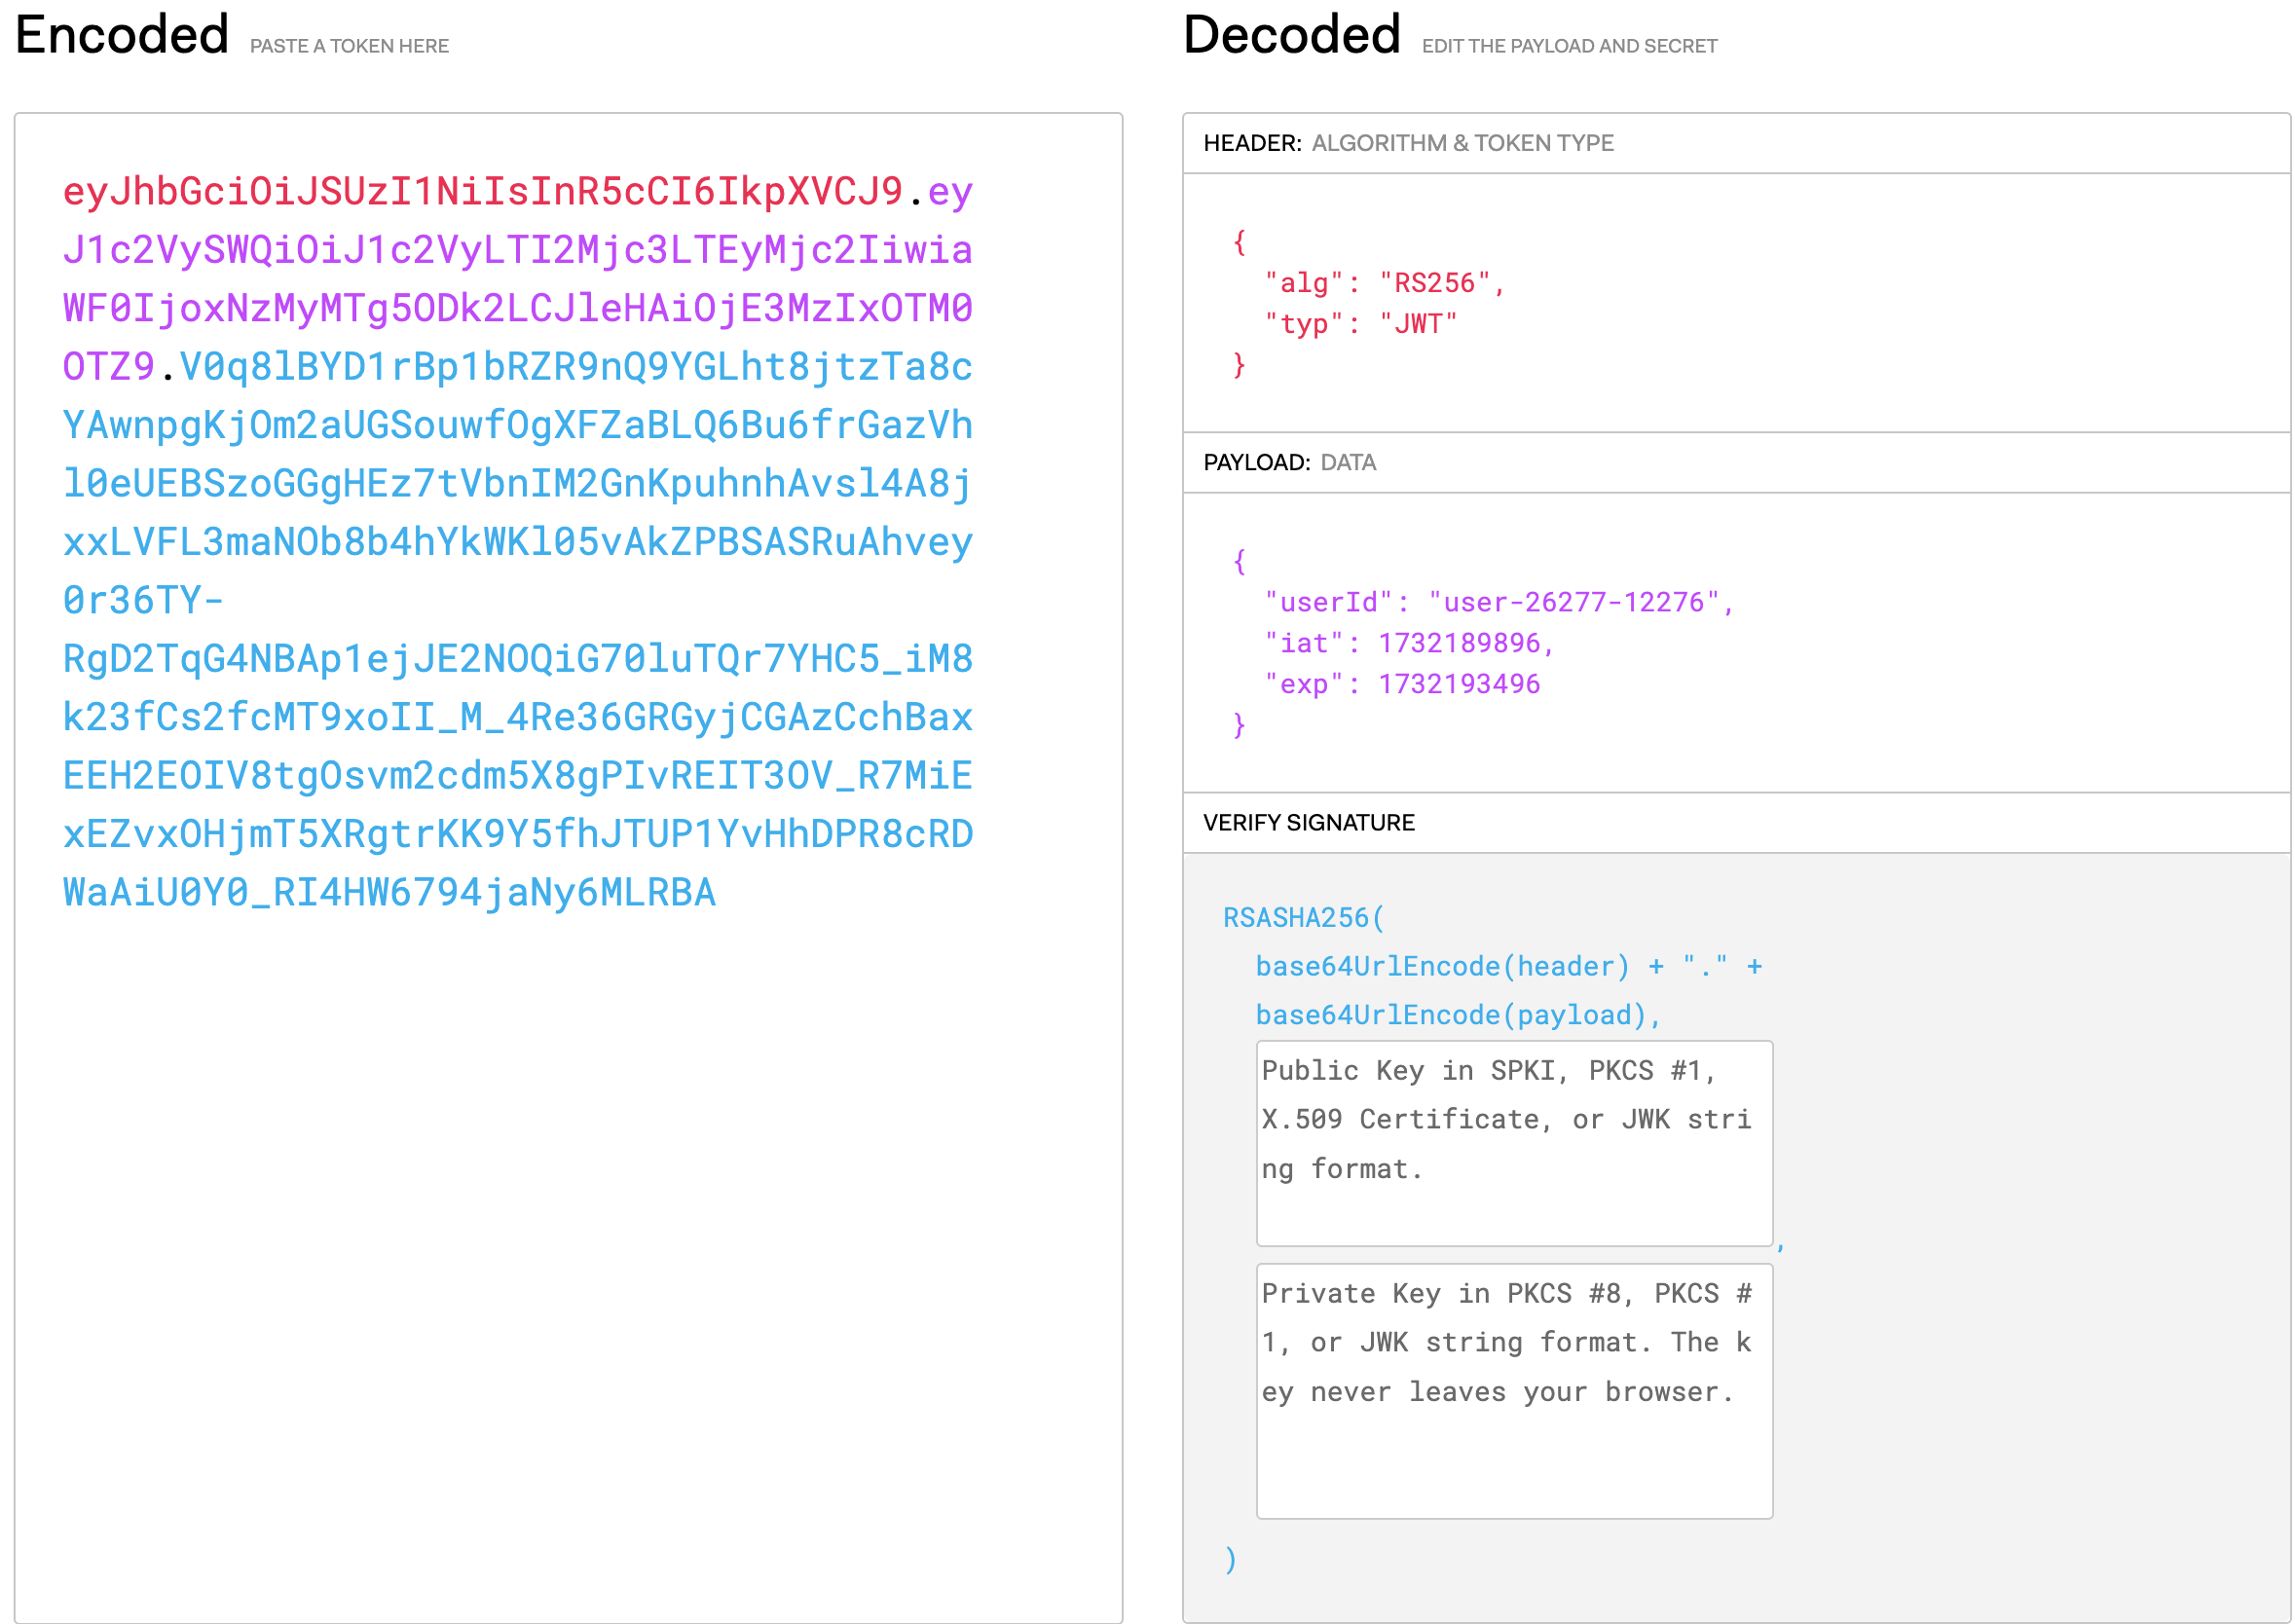
\includegraphics[width=\textwidth]{pics/token_signed.png}
    \caption{Signed Token with a symmetric key using RS256 for tamper protection}
    \label{fig:token_tenant_1_token_signed}
\end{figure}